\Chapter{割り算再考(前多)}


小学校以来習ってきた割り算の概念をもう一度考えてみると,実は数学の概念に
繋がっていることがわかります.高校生にでもわかるよう配慮して書いたつもりですが,*がついている項目は大
学1,2年を想定して,**がついている項目は大学3,4年を想定して書いています.


\Section{割り算とは}

始まりは小学生の問題です.

問題 6人を2人ずつのチームにわけました.この時,何チームできるでしょう.\\
\hspace{4cm} 式 $6 \div 2=3.$ \hspace{4cm} 答え\ 3チーム.\\
懐かしいですね.また,足し算の答えを「和」と言うように割り算の答えは,「商」と言うんでした.ちなみに$\div$という記号はアメリカ,日本,イギリスぐらいし
か使われておらず,標準的には$6/3$とスラッシュを使いますので,今回もこれ以降
は$/$で書きます.

さて,今回注目したいのは,式ではなく図です.

\begin{picture}(200,130)(0,0)
 \put(160,20){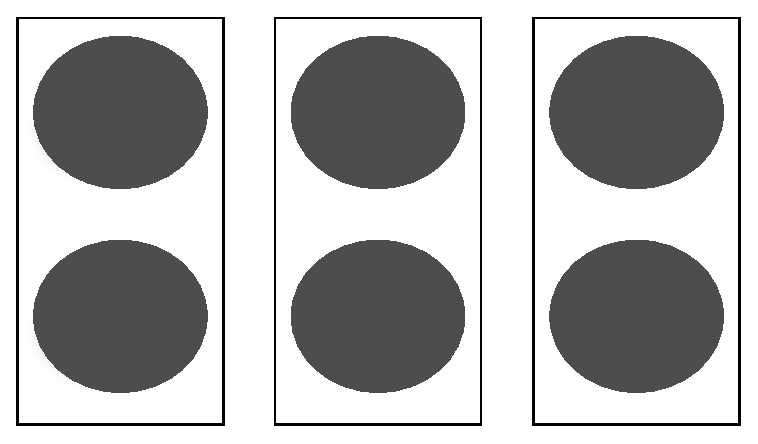
\includegraphics[scale=0.5, bb=0 0 1 1]{warizan1.eps}}
 \put(190,0){\text{図1\ :\ 3つのチーム分け}}
\end{picture}

小学校以来習ってきた割り算というのは,「たくさんあるものを,均等にチーム分けした
時のチーム数を求める演算」だと考えることができます.このイメージを
元に,「集合の割り算」を定義してみましょう.

\Section{商集合}

とはいえ,集合が与えられたとき,いきなり割り算するというのはできません.
「チーム分け」するには何が必要かを考えてみましょう.なお,大学以降では,
集合の要素のことを「元(げん)」というので,これ以降の記事では,要素を元と書くことにします.

\Subsection{同値関係}
チーム分けするためのアイディアは,「同じチームに属する条件」を与えるこ
とです.「同じチームに属している条件」を「同値関係」と言います.「同値関
係」は,以下に定義されるような3つの条件を満たす必要があります.

\begin{defi}[同値関係]
 集合$X$に対し,同値関係$\sim$とは,以下の3つの条件を満たす集合の元の間の関係をいう.
 \begin{enumerate}
  \item(反射律) 全ての$x\in X$に対し,$x \sim x.$
  \item(対称律)  $x\sim y$を満たす全ての$x,y\in X$に対し,$y\sim x$
  \item(推移律) $x\sim y$,$y\sim z$を満たす全ての$x,y,z\in X$に対し,$x\sim
	z$
 \end{enumerate}
\end{defi}
一見,難しそうな定義ですが,よく読めば大したことは言っていません.1つ目の条件は,どんな奴でも自分自身とは同じチーム,
2つ目の条件は,チームメートは逆からみてもチームメート,
3つ目の条件は,チームメートのチームメートはチームメートだと言うことです
(当然成り立ってほしい条件ですよね).


例をいくつかあげてみましょう.
\begin{Ex}
 自然数の集合$\mathbb{N}$において,元の関係$\sim$を
 \[
  n\sim m\Leftrightarrow n-mは2で割り切れる
 \]
 と定めると,これは同値関係です.実際,どんな数$n$についても,$n-n=0$は$2$で割り切れます
 し,$n-m$が$2$で割り切れるなら$m-n$も2で割り切れます.さらに,$n-m,m-l$
 が$2$で割り切れるなら$n-l$も2で割り切れます.今は「$2$」で割り切れると
 しましたが,他の自然数でも上のように定めれば同値関係になることは同様に
 示せます.
\end{Ex}


\begin{Ex}
 実数の集合$\mathbb{R}$において,$\leq(<または=)$で定められる元の関係
 \[
  x\sim y\Leftrightarrow x\leq y
 \]
 は同値関係ではありません.どんな実数$x$に対しても$x\leq x$です
 し,$x\leq y$かつ$y \leq z$ならば$x\leq z$ですから,反射律と推移律は満たしますが,対称律を満たしま
 せん.実際,$x\leq y$だからと言って,$y\leq x$とは限らないからです.
\end{Ex}

同値関係があるとき,同じチームに属している奴らを集めてきたものを,同値類と言います.例
えば,$x\in X$と同値関係にある$X$の元全体($x$が入っているチーム)を,$[x]$で書くことにします.
\[
 [x]=\{y\in X\ |\ x\sim y\}
\]
すると,集合を「チーム分け」する,つまり集合の割り算を定めることができま
す.

\Subsection{商集合の定義}

さて,同値関係が定まると集合の割り算を定義できます.

\begin{defi}[商集合]
 集合$X$とその上の同値関係
 $\sim$に対し,商集合$X/\mathord{\sim}$を以下で定める.
 \[
   X/\mathord{\sim}=\{[x]\ |\ x\in X\}
 \]
\end{defi}

例で感覚を掴みましょう.

 \begin{Ex}{\ } \\
  $X=\{0,1,2,3,4,5,6\}$とします.このとき,$X$に,同値関係$\sim$を,
 \[
  n\sim m\Leftrightarrow n-mが2で割り切れる
 \]
 と定めます.このとき,商集合$X/\mathord{\sim}$は何になるでしょうか.例えば,$1$
  の同値類($1$の入っているチーム)は,$[1]=\{1,3,5\}$, $0$の同値類は,$[0]=\{0,2,4,6\}$となります.こ
  れ以外のチームはありませんから,
  \[
    X/\mathord{\sim}=\{[0],[1]\}=\{\{0,2,4,6\},\{1,3,5\}\}
  \]
であるとわかります.まさに偶数と奇数への「チーム分け」ですよね.$\{0,1\}$
  はチームの代表メンバーであり,数学用語でも「完全代表系」と言います.しかし,
  わり算とはいえ,必ずしも1つ1つのチーム
  の元の数は一致しないことには注意しましょう.
 \end{Ex}

 \Section{様々な商集合の例}
\Subsection{合同式}
  まずは,上の概念をそのまま延長して自然数の集合$\mathbb{N}$に対して,同値
  関係$\sim$を以下で定めてみます.
  \[
   x\sim y\Leftrightarrow x-yが4で割り切れる
  \]
  この同値関係で割った集合$\mathbb{N}/\mathord{\sim}$は,4で割ったあまりでのチーム分けになり
  ます.
  \[
    \mathbb{N}/\mathord{\sim}=\{[0],[1],[2],[3]\}
  \]
  これを図にすると以下のようになります.自然数全体を4つのチームに分け
  てしまったのがよくわかると思います.\\
 \begin{picture}(200,150)(0,0)
   \put(200,20){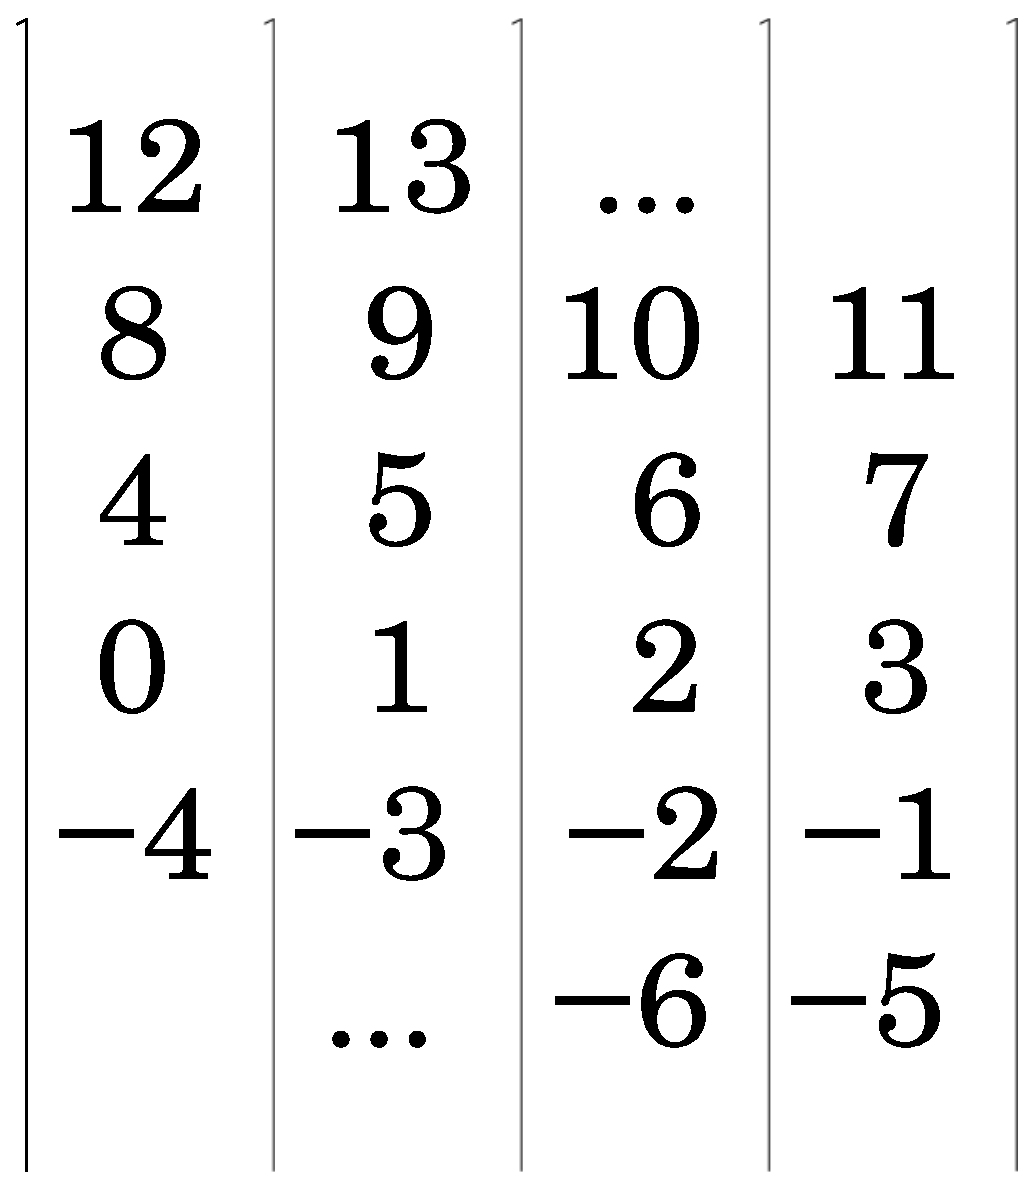
\includegraphics[scale=0.25, bb=0 0 1 1]{warizan2.eps}}
   \put(175,5){\text{図2\ :\ $4$で割ったあまりでチーム分け}}
 \end{picture}
 
  
  合同式を思い出してみましょう.
  \[
   1\equiv5  \mod4
  \]
  などという表記を見たことがあるかもしれませんが,これは,$1$と$5$が上で
  定めた同値
  関係,すなわち$1\sim 5$を示しているに他なりません.
  さらに,もともと$\mathbb{N}$に定まっている足し算,掛け算はそのまま
  $\mathbb{N}/\mathord{\sim}$に遺伝します.つまり,
  \[
   [a]+[b]=[a+b]\hspace{1cm}[a]\times[b]=[a\times b]
  \]
  が成り立つということです.これを使えば,例えば
  \[
   \bigl[15^{30}\bigr]=[15]^{30}=[3]^{30}=\bigl[3^2\bigr]^{15}=[1]^{15}=[1]
  \]
  となり,$15^{30}$がチーム$1$に属する(すなわち,4でわると1あまる)ことがすぐ確かめられます.

\Subsection{ベクトル}
今までは数字を使っていましたが,集合にしたおかげで,もっと概念的なものに
ついても商集合を考えることができます.高校で習うベクトルも,商集合として
考えてみましょう.
$E$を平面(もしくは空間)の有向線分(向きを持った線分,つまり矢印)全体から
なる集合とします.このとき,$E$上の同値関係を,
\[
 v\sim w\Leftrightarrow vとwは平行移動で重なる
\]
と定めます(同値関係になっていることはチェックしてみてください).このとき,
$E/\mathord{\sim}$がまさに平面全体のベクトルを集めた集合になります.この商集合の
 一つ一つの元は「平行移動で重なったら同じベクトルを集めたチーム」になります
 が,この中で原点を始点として持つものを「代表」とすれば,終点の「座
 標」で全てのチームが表せます.これこそがベクトルの「成分表示」なのです.

\Subsection{空間の貼り合わせ}
ベクトルの例からもわかるように,あるものたち(ベクトルの場合は平行移動し
たもの)を{\bf「おんなじものと見たい」「同一視したい」}と
いう気持ちがあるときは,商集合が使われます.数学においては図形同士を,のりで貼
り合わせたいというシーンに多々遭遇しますが,これをキチンと定式化するのも
商集合の大事な役割です.例えば,下の円と直線を黒点の部分で貼り合わせてみましょう.

\begin{picture}(150,100)(0,0)
 \put(150,10){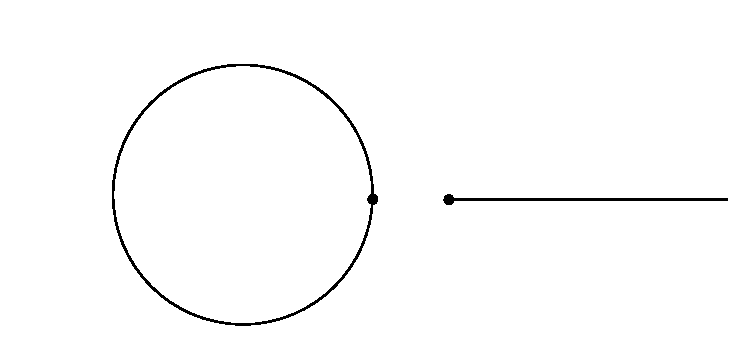
\includegraphics[scale=0.5, bb=0 0 1 1]{warizan4.eps}}
\end{picture}

このとき,二つの図形の点の集まりを一つの集合$X$だと考え,$A$を2つの黒点からなる集合として,以下のよう
な同値関係を定めます(同値関係になっていることはすぐ確かめられます).
\[
 x\sim y\Leftrightarrow 
			x,y \in Aまたは
			x=y 
\]
つまり,$A$に入っていない点たちは,その点1点からなるチームに,$A$に入っ
ている点たちはまとめて一つのチームにしてしまいます.そうすれば,チーム全
体の集合$X/\mathord{\sim}$は,まさに,二つの図形を貼り付けたものになっていることがわかりま
す.
このような貼り付けにより作られる図形の一つをみてみましょう.正方形の辺を貼り付けて立体を作るということを考えてみます.図の黒点同士のように,左側の辺と右
側の辺,上と下も同様に,同じ方向に貼り付けると,右のように浮き輪の形の図
形が出来上がります.これは(2次元)トーラスといい,数学の様々な場面に登場
します.

\begin{picture}(400,120)(0,0)
 \put(40,10){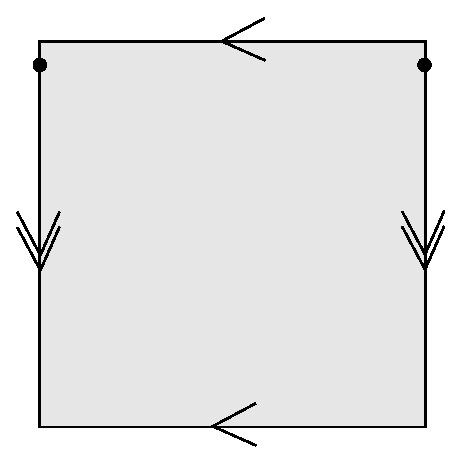
\includegraphics[scale=0.5, bb=0 0 1 1]{warizan3.eps}}
 \put(150,55){\text{\huge $\Rightarrow$}}
 \put(175,30){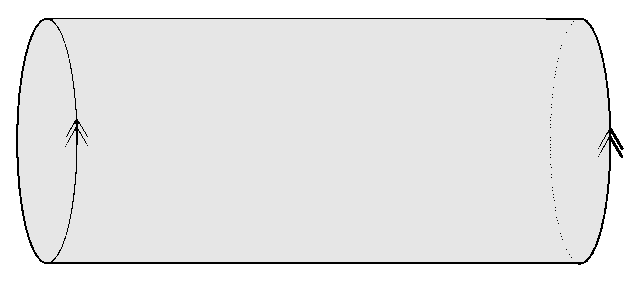
\includegraphics[scale=0.5, bb=0 0 1 1]{warizan5.eps}}
 \put(325,55){\text{\huge $\Rightarrow$}}
 \put(350,30){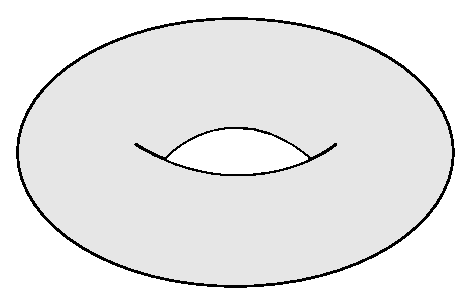
\includegraphics[scale=0.5, bb=0 0 1 1]{torus.eps}}
 \end{picture}

ちなみに,貼り付けかたを一つだけ逆にすればクラインの壺,二つとも逆に
すると二次元射影空間と呼ばれる図形になります(想像できますか?).\\
二次元球面(地球の表面)は地球上の地図を貼り合わせて構成できますし,多くの図形は
貼り合わせによって構成が可能です.大雑把に言って,このように直線や平面な
どまっすぐな空間を貼り合
わせて作られる図形のことを数学では多様体と呼び,古くから研究されてきた対
象です.

\Subsection{商ベクトル空間*}
ここで扱う例は,大学1年生で習うベクトル空間の概念なので,知らない人は
飛ばしてもらって結構です.\\

ここまでの概念がわかってしまえば,大学1年生の線形代数での1つの難所である
商空間は簡単に定義できます.

\begin{defi}
 ベクトル空間$V$と部分空間$W$に対し,$V$上の同値関係を,
 \[
  v_1\sim v_2\Leftrightarrow v_1-v_2\in W
 \]
 と定義する.$V/\mathord{\sim}$を,部分空間$W$による$V$の商空間といい,$V/W$で表す.
\end{defi}

これだとイメージしにくいかもしれませんが,$v_1$の同値類$[v_1]$は
$v_1+w\ (w\in W)$
と書けるものな訳ですから,$W$の元だけずれているものは全て同じチームなの
です.絵で描けば,以下のようになります.まず,部分空間とは,原点を通るまっ
すぐな空間ですから,$V$と$W$の図は以下のようになります.\\
\begin{picture}(400,150)(0,0)
 \put(150,10){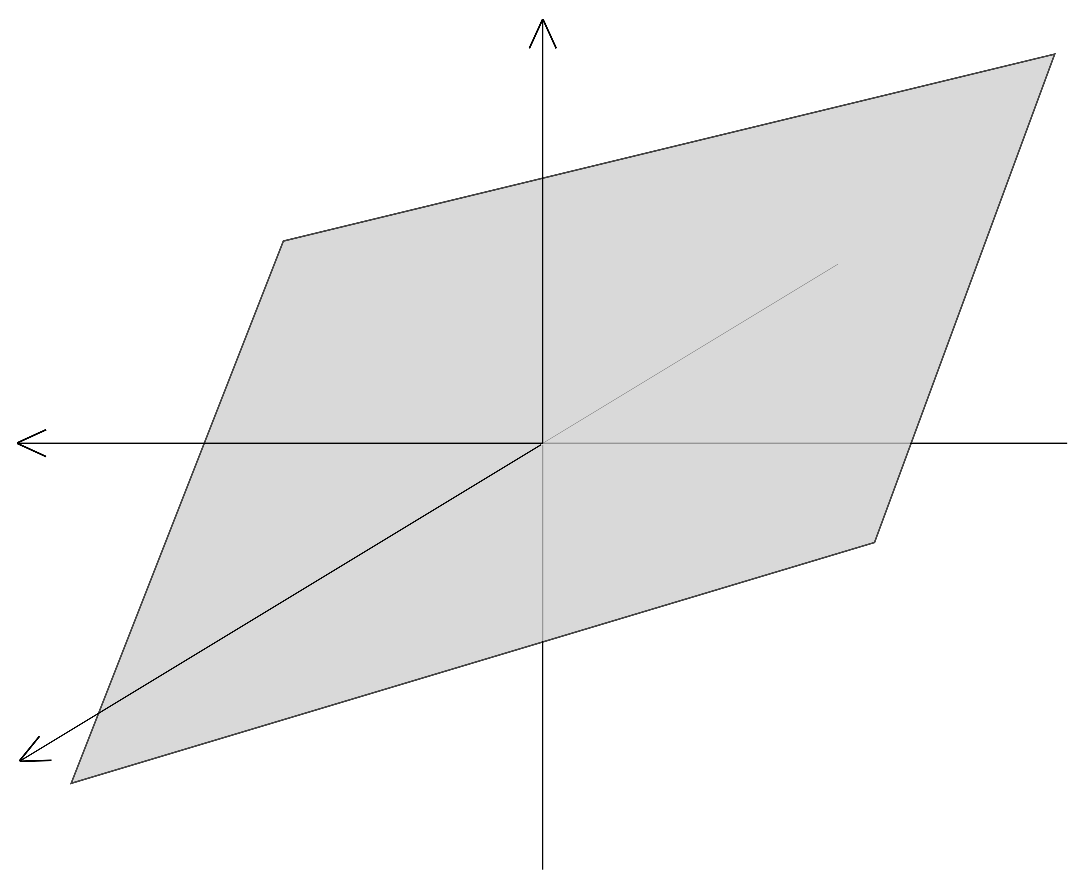
\includegraphics[scale=0.4, bb=0 0 1 1]{warizan6.eps}}
 \put(260,100){\text{$W$}}
\end{picture}

この空間$W$全てが同じチームとなりますので,チームは以下
のようにならんでいることがわかります.つまり,商空間とは,この1枚1枚のチームの全体となるの
です.完全代表系は,$W$と原点のみにおいて交わる直線と平面たちの交点となり
ます(完全代表系の取り方は無限通りあります).つまり,商空間$V/W$はこの直線と同
一視できるのです.スカラー倍や足し算については合同式のときと同じく商集合に遺
伝することが示せるので,$V/W$もベクトル空間となることがわかります.
イメージとしては,商空間$V/W$は$V$を図の直線に向かって潰した空間というこ
とになります.潰した時,$W$は原点に潰れるわけですから,$V$において,$W$
の成分を全て$0$と同一視したものだとも言えます.


\begin{picture}(400,150)(0,0)
 \put(150,10){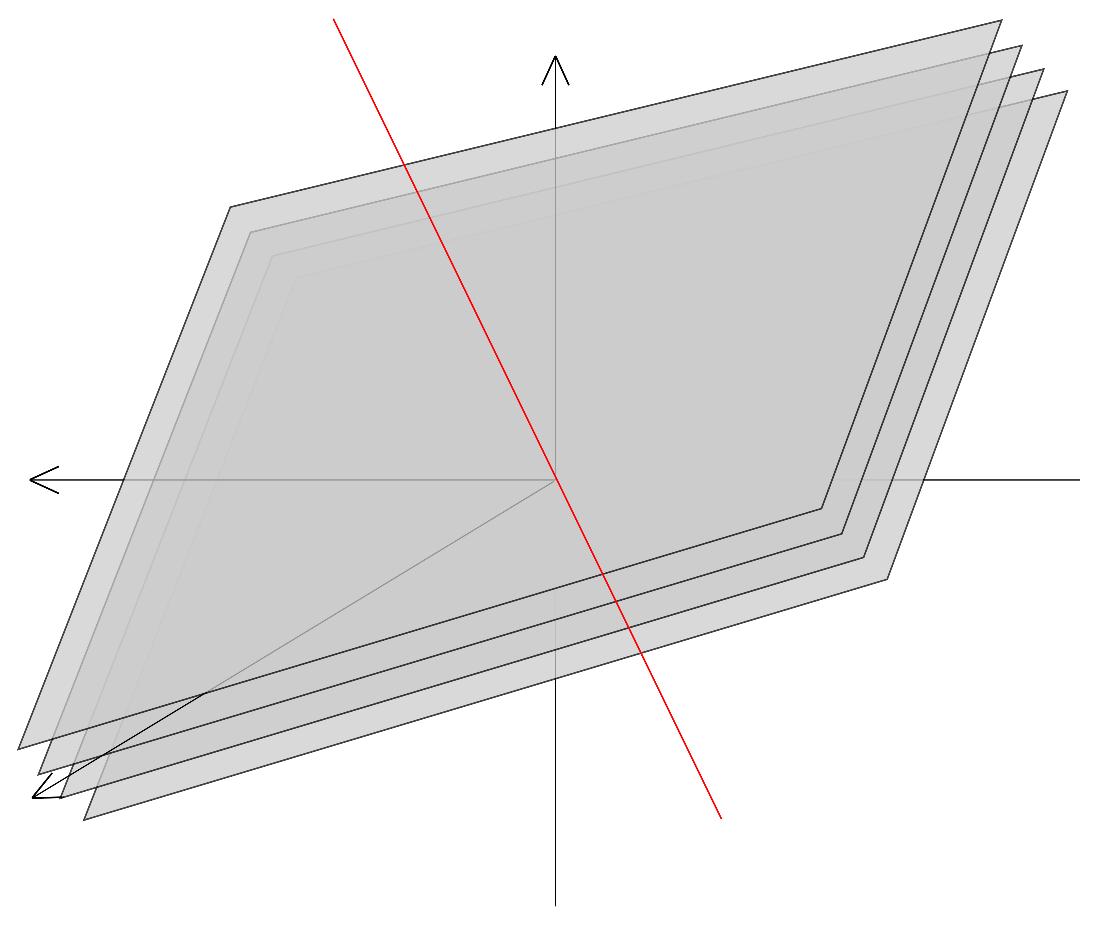
\includegraphics[scale=0.4, bb=0 0 1 1]{warizan7.eps}}
\end{picture}
\Section{数の構成}

さて,ここからは応用編です.唐突ですが,「整数,有理数,実数とは何か」と聞かれ
たとき,何て答えるでしょうか.「え,そりゃあ,$-1$とか分数とかでしょ?」
とか答えられても,あくまでそれは例にすぎません.「自然数の集合
$\mathbb{N}$と足し算,掛け算しか知らない」と仮定
して,整数の集合$\mathbb{Z}$や有理数の集合$\mathbb{Q}$,実数の集合$\mathbb{R}$を自然数のみを用いて構成してみ
ることにします.(今回は,自然数の存在は暗に認めています.公理的集合論の
立場では自然数は無限公理を満たす最小の集合として存在を保証しているのですが,今回は解説しないことにし
ます.)\footnote{以下の話の厳密な証明が知りたい場合,\cite{mathpdf}を参照してください.}

\Subsection{自然数から整数}

さて,自然数から整数を構成することを考えてみましょう.一番簡単なアイディ
アは,プラスパートとマイナスパートの自然数を作るということです.$(a,b)$と書
いたとき,1つめの項はプラス,2つ目の項はマイナスに当たると考えてみましょ
う.例えば,$(2,0)$を$2$に当たる数として,$(0,3)$を$-3$に当たる数として定めるわけです.そして,2つの数
の足し算を$(2,0)+(0,3)=(2,3)$と定めます.$(2,3)$はプラスパートとマ
イナスパートがそれぞれ$2,3$ですから,$-1$を表していると考えます.これで一見,うまくいっ
たかのように見えますが,これだと$(2,3)$と$(0,1)$が同じ数字を表しているた
め,”ダブり”が生じています.$(2,3)$と$(0,1)$を同じものと見たい,同一視し
たい.こんな時こそ商集合の出番です.


\begin{defi}[整数]
 自然数を二つ並べた集合$\mathbb{N}^2=\{(a,b)\ |\ a,b\in
\mathbb{N}\}$を考え,$\mathbb{N}^2$上に同値関係
\[
 (a,b)\sim(c,d)\Leftrightarrow a+d=b+c
\]
と定め,この同値関係による商集合$\mathbb{N}/\mathord{\sim}$を整数$\mathbb{Z}$と
 定める.
 さらに,$\mathbb{Z}$上の加法と乗法を,
 \[
  [(a,b)]+[(c,d)]=[(a+b,c+d)]\hspace{1cm}[(a,b)]\times[(c,d)]=[(ac+bd,ad+bc)]
 \]
 と定める\footnote{本当は,これで矛盾なく定まっていることをチェックしなければいけません.つまり,$(a,b)\sim(a',b')$のとき,\[(a+c,b+d)\sim(a'+c,b'+d)\hspace{1cm}(ac+bd,ad+bc)\sim(a'c+b'd,a'd+b'c)\]であることを示す必要があります.もしこうでなければ,足し算や掛け算の結果が,チームの代表メンバーの選び方によって違う結果になってしまい,矛盾してしまうからです.一つ目だけチェックすれば,$a+b'=a'+b$より$(a+c)+(b'+d)=(a'+c)+(b+d)$ですからうまくいっています(二つ目もチェックしてみましょう).このようにうまく定まっていることを,数学では,well-definedと言います.}
\end{defi}

例えば,$2+1=3+0$ですから,$[(2,3)]=[(0,1)]$だとわかりま
す.
掛け算はちょっと技巧的ですが,これでうまくいっていることがわかります.例
えば,正の数同士は,$[(n,0)]\times[(m,0)]=[(nm,0)] $と,今までと全く同じ
演算であることがわかります.また,$[(n,0)]\times[(0,m)]=[(0,nm)]$や,
$[(0,n)]\times[(0,m)]=[(nm,0)]$などから,プラスかけるマイナスがマイナ
ス,マイナスかけるマイナスがプラスであることも説明できます.\\
最後に,$[(x,0)]$を$x$とかき,$[(0,x)]$を$-x$を書くことにすれ
ば,今まで使っていた表記と合致します.


\Subsection{整数から有理数}

さて,今度は有理数を構成してみましょう.さっきのアイディアをそのまま借用
して,分母パートと分子パートを並べて書いてみることにします.つまり,
$(a,b)$と書いたとき,$\ds\frac{a}{b}$を表すとしてみます.しかし,分数と
いうのは,小学校以来,約分しても同じ,だったわけですから,例えば$(2,4)$
と$(1,2)$は同じものであってほしいわけです.そこで,商集合を使って同一視
してみます.

\begin{defi}[有理数]
$\mathbb{Z}\times(\mathbb{Z}-\{0\})=\{(a,b)\ |\
 a\in\mathbb{Z},b\in\mathbb{Z}-\{0\}\}$上に同値関係
 \[
  (a,b)\sim(c,d)\Leftrightarrow ad=bc
 \]
 と定め,この同値関係による商集合
 $\mathbb{Z}\times(\mathbb{Z}-\{0\})/\mathord{\sim}$を有理数$\mathbb{Q}$と定める.
 さらに,$\mathbb{Q}$上の加法と乗法を,
 \[
  [(a,b)]+[(c,d)]=[(ad+bc,bd)]\hspace{1cm}[(a,b)]\times[(c,d)]=[(ac,bd)]
 \]
 と定める\footnote{これもwell-definedであることをチェックする必要があります.示してみてください.}.
\end{defi}

$\sim$の同値関係は,外項と内項の積が等しい,つまり,$a:b=c:d$を表していますから,同じ分数を1チームにまとめていることがわかります.\\
さて,定義から,$[(1,1)]$はどんな数とかけても相手を変えない,自然数の''1''に当たる数だとわかります.また,$[(0,1)]$は,どんな数とかけても$[(0,1)]$になり,どんな数と足し算しても相手を変えない,自然数の''0''に当たる数だとわかります.\\
また,
\[
 [(a,b)]\times[(b,a)]=[(ab,ab)]=[(1,1)]
\]
ですから,$[(a,b)]$に,$[(b,a)]$をかけると1になることがわかります.
ということは,
\[
 [(c,d)]=[(a,b)]\times([(b,a)]\times[(c,d)])
\]
ですから,
\[
 [(c,d)]/[(a,b)]=[(b,a)]\times[(c,d)]
\]
となり,小学校以来やってきた,分数の割り算は分母と分子をひっくり返してかけるということも正当化できます.

最後に,$(a,b)$を$\ds\frac{a}{b}$と書く\footnote{ちなみに,$\ds\frac{a}{b}$は日本語では「$b$分の$a$」と読みますが,英語では逆で,''$a$ over $b$''と読みます.}ことにすれば,今まで使っていた表記と合致します.

\Subsection{有理数から実数}

さて,最後に実数を作ってみましょう.これはかなり困難です.実数の構成には,代表的なものでDedekind cutによるものと,有理数の完備化の二つがあるのですが,今回は有理数の完備化を解説したいと思います.
\begin{defi}[Cauchy列]
 数列$\{a_n\}$がCauchy列であるとは,以下のことを言う.
 \[
  \forall \varepsilon >0 \ \exists N\  {\rm such\ that}\ n,m>N \Rightarrow |a_n-a_m|<\varepsilon
 \]
\end{defi}
一見ギョッとするような定義ですが,簡単に言えば,コーシー列とは,「二項間の差がどんどん小さくなっていくような数列」のことです.
さて,ここで,次のような問題を考えて見ましょう.
\begin{center}
 Cauchy列は収束するでしょうか?
\end{center}
答えは,実数列なら○,有理数列なら×です.数学用語でこの性質を「完備性」と言います.有理数は完備ではないのです.例えば,有理数で$\sqrt{2}$に近づくような数列を考えてみれば,もちろん二項の差は縮まっていきますが,肝心の収束先の$\sqrt{2}$が有理数ではないですから,「有理数の中では」収束しません.このことに着目して,有理数から実数を作ります.具体的には,
\begin{center}
  $\sqrt{2}$ に収束する有理数列を $\sqrt{2}$ だと定義する
\end{center}
です.数列と $\sqrt{2}$ を同じと見るなんてかなり気持ち悪いですが,一応定義はできるわけです.とはいっても,$\sqrt{2}$に収束する有理数列はいっぱいあります.そこで,商集合の考え方を使って,$\sqrt{2}$に収束する数列を1チームにしてしまえば良いのです.
\begin{defi}[実数]
$\mathcal{C}$を有理数のCauchy列全体からなる集合とし,$\mathcal{C}$上の同値関係を,
 \[
 \{a_n\}\sim\{b_n\}\Leftrightarrow \forall\varepsilon\  \exists N\  {\rm such\ that}\ n>N\Rightarrow |a_n-b_n|<\varepsilon
 \]
 と定め\footnote{これが同値関係であることは非自明ですが,ここでは省略します.},この同値関係による商集合$\mathcal{C}/\mathord{\sim}$を実数$\mathbb{R}$と定める.さらに,$\mathbb{R}$上の加法と乗法を,
 \[
  [\{a_n\}]+[\{b_n\}]=[\{a_n+b_n\}]\hspace{1cm}[\{a_n\}]\times[\{b_n\}]=[\{a_nb_n\}]
 \]
 と定める.\footnote{これがwell-definedであることも非自明ですが,ここでは省略します.}
\end{defi}

上のように定めれば$\{a_n\}\sim\{b_n\}$であれば,$\{a_n\}$と$\{b_n\}$が同じ値に近づいていくことがわかります.
本当は,$\mathbb{R}$が満たすべきたくさんの性質をここから示さなければいけないのですが,今回の主題はそこではないので,詳しくは参考文献を見てみてください.

このように,存在が当たり前だと思っていた整数や有理数や実数,そしてそのたくさんの性質は,商集合のアイディアに支えられているのです.\footnote{実は複素数も,商集合を用いて$k[X]/(X^2+1)$などと定義できるのですが,今回は紙面の関係上,省略します.}


\Section{応用**}
最後に,少しだけ応用をみてみます.
 \Subsection{等質空間}
群構造をもつ可微分多様体で群の積演算$(a,b)\mapsto ab$と逆演算$a\mapsto a^{-1}$が可微分であるものをLie群と言います(群と多様体のあいのこです).例えば,一般線形群$GL(n,\mathbb{R})$や特殊線形群$SL(n,\mathbb{R})$,特殊直交群$SO(n)$などはLie群になっています.

さて,Lie群$G$がある多様体$M$に推移的に作用していることを考えてみましょう.推移的,というのは全ての点同士があるLie群の元の作用で写りあえるという意味です.全射群準同型$G\rightarrow \rm{Diff}(M)$があると言ってもいいです.
例えば,球面$S^n$,上半平面$H$には,
\begin{eqnarray*}
SO(n+1)&\rightarrow & {\rm Diff}(S^{n})\hspace{1cm}A\mapsto (p\mapsto Ap)  \\
SL(2,\mathbb{R})&\rightarrow & {\rm Diff}(H)\hspace{1cm}\left(\begin{matrix}a&b\\c&d\end{matrix}\right)\mapsto\left(z\mapsto\frac{az+b}{cz+d} \right) 
 \end{eqnarray*}
のように,Lie群が推移的に作用しています.
この時,ある一点$p$の群作用による行き先(軌道)は,推移的であるという仮定から全体を覆うわけですが,作用させても動かない$G$の元があるかもしれません.これを集めたもの,
\[
 H=\{g\in G\ |\ gp=p\}
\]
を$G$の一点$p$の固定部分群と言います(定義より閉部分群になります).
この$H$たちをチームにして, 点$p$と同一視すれば,作用させている空間との1対1対応ができます.
すなわち,
\[
 G/H\simeq M\hspace{1cm}[g]\mapsto gp
\]
となるわけです.

ここで,左辺の$G/H$とは,$G$を,$g_1\sim g_2\Leftrightarrow g_1g_2^{-1}\in H$という同値関係で割ったもので,$G$の部分群$H$による商群と呼ばれます.特に,Lie群をその中の閉部分群で割った商群$G/H$には多様体構造が定まることが知られており,上の同型は微分同相であることが示せます.

このように,Lie群が推移的に作用している多様体は,必ずLie群の商の形で書くことができます.このような多様体を等質空間と言います.

\begin{Ex}[球面]
 $SO(n+1)$の作用による球面$S^n$上のある1点$(0,0,0,\cdots,0,1)$の固定部分群は,
 \[
\left\{
\left(
\begin{array}{ccc:c}
&&&\\
&\mbox{\smash{\huge\textit{A}}}&&{{0}}\\
&&&\\ \hdashline
&0&&1
\end{array}
\right) \middle|\ A\in SO(n) \right\}\simeq SO(n)
 \]
よって,$S^n\simeq SO(n+1)/SO(n)$となります.
\end{Ex}

\begin{Ex}[上半平面]
$SL(2)$の作用による上半平面$H$上のある1点 $i$ ($=\sqrt{-1}$) の固定部分群は,
 \[
  \frac{ai+b}{ci+d}=i\Leftrightarrow a=d,\ b=-c
 \]
より,
 \[
  \left\{\left(\begin{matrix}
   a&b\\c&d
  \end{matrix}\right)\in SL(2,\mathbb{R})\ \middle|\  a=d,b=-c\right\}\simeq SO(2)
 \]
よって,$H\simeq SL(2,\mathbb{R})/SO(2)$となります.$H$は複素多様体ですが,実Lie群の商でかけます.
\end{Ex}

この表示の一つのメリットは,ある1点に定めた幾何構造を全体に写すことにあります.
$G/H$の形で書いた場合,当然,原点の同値類$[e]$があります.
これについて
\begin{Lemma}\label{l4}
  $G/H$を等質空間とする.集合として,次の同型がある.
 \[
  (\bigotimes^rT_{[e]}M\otimes\bigotimes^sT^*_{[e]}M)^H\simeq (\Gamma(M,\bigotimes^rTM\otimes\bigotimes^sT^*M))^G
 \]
 ただし,左は,$\Ad(H)$不変なテンソルの元,右辺は$M$からベクトル束への左作用の微分${L_{G}}_*$不変な切断である.
 \end{Lemma}
表示は仰々しいですが,例えば,$r=1,s=0$とすれば,$H$不変な接空間のベクトルと,$G$不変なベクトル場が1対1に対応していることがわかりますし,$r=0,s=2$とすれば,$H$不変な接空間上の内積と,$G$不変な計量,$H$不変な複素構造と$G$不変な概複素構造が1対1に対応することがわかります.\\
他にも,等質空間上では測地線をLie代数からLie群への指数写像でかけたり,曲率テンソルが,Lie括弧でかなりシンプルにかけたりなど,計算できる具体例を豊富に提供してくれます.


\Subsection{Clifford-Klein形}
Riemannの一意化定理の一般化である,Klein-Poincar\'e-Koebeの一意化定理より,Riemann面の普遍被覆は,上半空間$H$,複素数$\mathbb{C}$,複素射影空間$\mathbb{P}^1$のいずれかに正則同値になります.また,特に,種数が2以上のコンパクトRiemann面は,上半平面を,Fuchs群と呼ばれる$\rm{Aut}(H)$の離散部分群$\Gamma$で割って作られます.$H$自体は上で見たように$SL(2,\mathbb{R})/SO(2)$とかけますから,コンパクトRiemann面は,$\Gamma\backslash SL(2,\mathbb{R})/SO(2)$という$SL(2,\mathbb{R})$を2回割ったものとして書くことができます.一般に,$G/H$に固有不連続かつ自由に作用する$G$の離散部分群$\Gamma$が存在すれば,等質空間$G/H$をさらに割った$\Gamma\backslash G/H$を考えられます.これをClifford-Klein形といい,等質空間より豊富な例を含む広いクラスとして,現在も研究されています.

{\bf 終わりに}\\
たくさんの例を「割り算」というテーマでざっくばらんに解説してみました.何を隠そう,この集合の割り算という概念を理解するのに僕自身苦労したので,あえて書いて見ました.数学というと,「イメージではなく,論理的にのみ考える学問」と考えられがちな気がします.論理ももちろん大事ですが,決して論理だけではなく,むしろ,「イメージをいかに数式という形で正確に伝えられるか」というモチベーションで研究が進むことも多いと思います.高校や大学で難しい概念に出会ったときは,ただ定義を眺めるだけではなく,様々な例を見ながら,どういう気持ちで概念が生まれているのかを考えて見るといいと思います.

\begin{thebibliography}{99}
\bibitem{mathpdf} 数の構成 自然数から複素数まで \url{http://mathematics-pdf.com/pdf/construction_of_numbers.pdf}
\bibitem{hel} S.Helgason.Differetntail Geometory and Symmetric Spacees.AMS Chelsea Publishing,2001
\bibitem{sat} 佐武一郎.線型代数学.裳華房,数学選書1,1974
\bibitem{mat} 松坂和夫.集合・位相入門.岩波書店,1968
\bibitem{kob} 小林俊行.数学の最先端21世紀への挑戦.vol1.Springer,2001
\end{thebibliography}
